\documentclass[conference]{IEEEtran}
\IEEEoverridecommandlockouts
\usepackage{cite}
\usepackage{amsmath,amssymb,amsfonts}
\usepackage{algorithmic}
\usepackage{graphicx}
\usepackage{textcomp}
\usepackage{xcolor}
\usepackage{hyperref}
\usepackage{placeins}
\usepackage[spanish, mexico]{babel}
\def\BibTeX{{\rm B\kern-.05em{\sc i\kern-.025em b}\kern-.08em
    T\kern-.1667em\lower.7ex\hbox{E}\kern-.125emX}}
\usepackage[table,xcdraw]{xcolor}

\title{Aplicación de Redes Neuronales Convolucionales para la Clasificación de Imágenes}

\author{\IEEEauthorblockN{
Dora Alicia Guevara Villalpando \\
Matrícula: 1551003}
\\
\IEEEauthorblockA{\textit{Universidad Autónoma de Nuevo León)} \\
\textit{Facultad de Ciencias Físico Matemáticas}\\
Maestría en Ciencia de Datos \\
Procesamiento y Clasificación de Datos\\\\
dora.guevaravll@uanl.edu.mx}
}

\date{\today}


\graphicspath{{./imagenes_reporte/}}  % Carpeta donde se guardan las imágenes


\begin{document}

\maketitle


\begin{abstract}

Este trabajo presenta una aplicación de redes neuronales convolucionales (CNN) para la clasificación de imágenes en tres categorías: aves, gatos y perros. Se empleó el preprocesamiento de datos mediante normalización y aumento de datos para mejorar la capacidad de generalización del modelo. La red neuronal fue entrenada con el optimizador \texttt{Adam} y la función de pérdida  \texttt{categorical crossentropy}. Los resultados obtenidos muestran una precisión de validación del 86\% en las mejores iteraciones, lo que indica un buen desempeño del modelo en la tarea de clasificación.

\end{abstract}



\section{Introducción}

Las redes neuronales convolucionales han demostrado ser altamente eficaces en tareas de visión por computadora, como la clasificación de imágenes, la detección de objetos y la segmentación. En este proyecto, se desarrolla un modelo CNN para la clasificación de imágenes de animales en tres clases distintas. La aplicación de técnicas de preprocesamiento y aumento de datos permite mejorar la robustez del modelo, evitando el sobreajuste y aumentando su capacidad de generalización.

El objetivo de este trabajo es evaluar el desempeño de un modelo CNN en la clasificación de imágenes de animales y analizar el impacto del preprocesamiento y el aumento de datos en su precisión y capacidad de generalización.

\FloatBarrier

\begin{figure}[h]
    \centering
    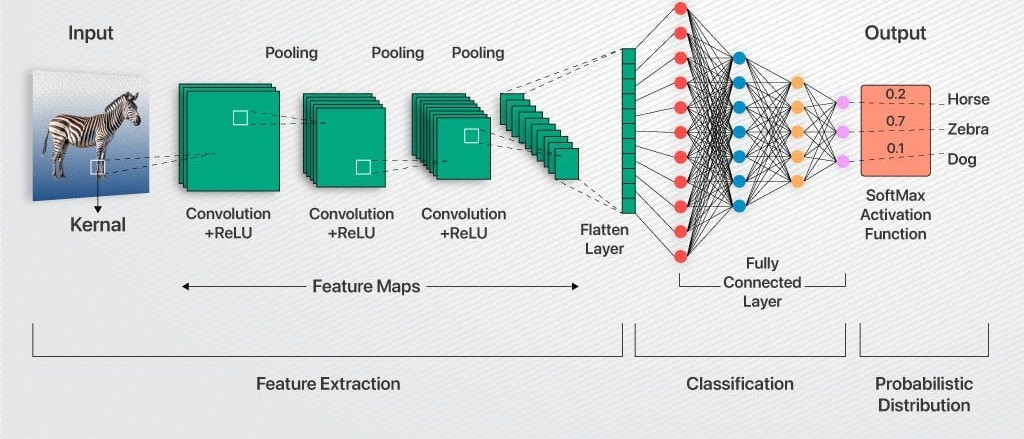
\includegraphics[width=.45\textwidth]{cnn_structure.jpg}
    \caption{Ejemplo de una red neuronal convolucional.}
    \label{fig:cnn_structure}
\end{figure}

\FloatBarrier



\section{Metodología}


\subsection{Preprocesamiento de datos}

\begin{itemize}
    \item \textbf{Organización del conjunto de datos:} Se recopilaron imágenes de las categorías aves, gatos y perros, las cuales fueron organizadas en carpetas para facilitar su uso en entrenamiento y prueba.

    \item \textbf{División de datos:} Se estableció una proporción del 80\% de las imágenes para entrenamiento y 20\% para prueba.

    \item \textbf{Normalización de imágenes:} Los valores de los píxeles fueron escalados dividiéndolos por 255, lo que ayuda a mejorar la eficiencia del entrenamiento al reducir la variabilidad numérica.

    \item \textbf{Verificación de imágenes:} Se implementó un proceso para identificar imágenes corruptas o con formatos incompatibles, asegurando que solo se usaran imágenes válidas.
\end{itemize}



\subsection{Aumento de datos}

\begin{itemize}
    \item \textbf{Transformaciones aplicadas:} Se utilizaron técnicas como rotaciones aleatorias, desplazamientos horizontales y verticales, cambios de escala y volteos horizontales para incrementar la variabilidad en los datos.

    \item \textbf{Propósito del aumento de datos:} Ayuda a mejorar la capacidad de generalización del modelo y a reducir el sobreajuste.
\end{itemize}

En la figura \ref{fig:data_augmentation} se muestra un ejemplo de como queda la imagen después del aumento.

\FloatBarrier

\begin{figure}[h]
    \centering
    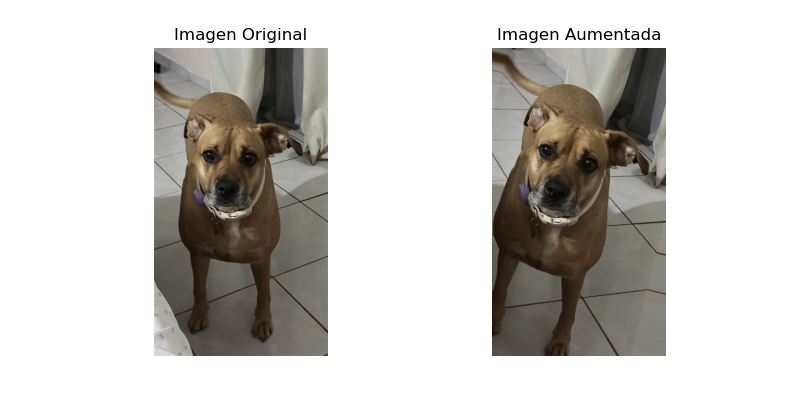
\includegraphics[width=.5\textwidth]{augmented_example.png}
    \caption{Ejemplo de imagen original y transformada con aumento de datos.}
    \label{fig:data_augmentation}
\end{figure}

\FloatBarrier



\subsection{Arquitectura del modelo}

\begin{itemize}
    \item \textbf{Capas convolucionales:} Se utilizaron tres capas convolucionales con activación \textit{ReLU}, cada una seguida de una capa de \textit{max-pooling} para reducir la dimensionalidad.

    \item \textbf{Capas densas:} Se agregaron capas completamente conectadas con activación \textit{ReLU} y una capa de salida con activación \textit{softmax} para la clasificación en tres categorías.

    \item \textbf{Regularización:} Se implementó una capa de \textit{Dropout} para reducir el sobreajuste.
\end{itemize}



\subsection{Entrenamiento y validación}

\begin{itemize}
    \item \textbf{Hiperparámetros:} Se configuró el entrenamiento con 100 épocas, un tamaño de lote de 16 y el optimizador \textit{Adam}.
    
    \item \textbf{Función de pérdida:} Se utilizó \textit{categorical crossentropy} para medir la diferencia entre las predicciones y las etiquetas reales.

    \item \textbf{Monitoreo del entrenamiento:} Se registraron la precisión y la pérdida en cada época para evaluar la evolución del modelo.
\end{itemize}



\section{Resultados}

\begin{itemize}
    \item La precisión en el conjunto de entrenamiento aumentó progresivamente, alcanzando valores superiores al 80\% en algunas épocas.
    
    \item La precisión de validación alcanzó un valor máximo de 86\%.

    \item La función de pérdida disminuyó de manera constante tanto en entrenamiento como en validación.

    \item Se generaron gráficas de evolución de precisión y pérdida.
\end{itemize}

\FloatBarrier

En la figura \ref{fig:training_curves} se muestra la evolución de la precisión y la pérdida durante el entrenamiento.

\begin{figure}[h]
    \centering
    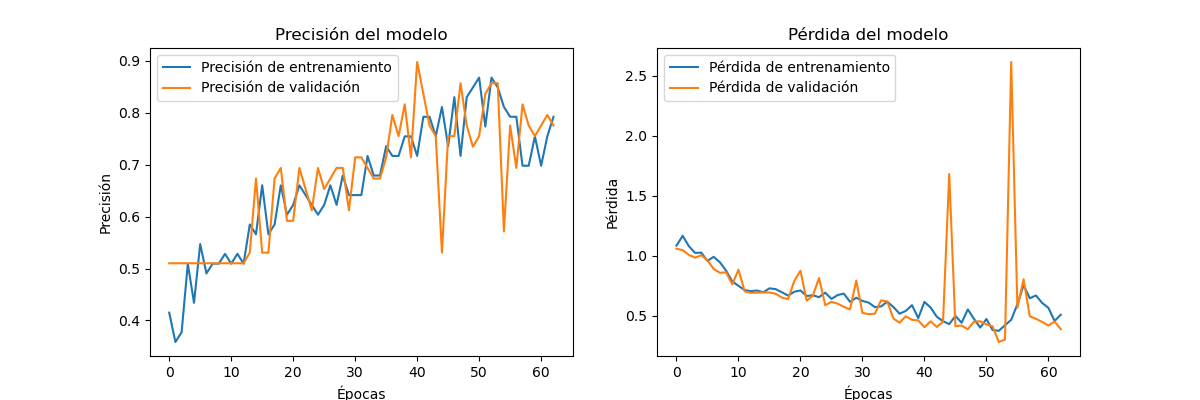
\includegraphics[width=.5\textwidth]{accuracy_loss_curve.png}
    \caption{Curvas de precisión y pérdida durante el entrenamiento.}
    \label{fig:training_curves}
\end{figure}

\FloatBarrier



\section{Conclusiones}

El modelo CNN desarrollado demostró ser efectivo en la clasificación de imágenes de animales, alcanzando una alta precisión en la validación. El uso de técnicas de preprocesamiento y aumento de datos contribuyó a mejorar la capacidad de generalización del modelo. Para futuras mejoras, se podría aumentar el volumen de datos de entrenamiento o utilizar arquitecturas preentrenadas para optimizar el rendimiento del modelo. En general, los resultados obtenidos validan la eficacia de las CNN en problemas de clasificación de imágenes.


En la figura \ref{fig:predictions} se muestra la clasificación de una imagen que no formo parte de la base inicial de imágenes.

\FloatBarrier

\begin{figure}[h]
    \centering
    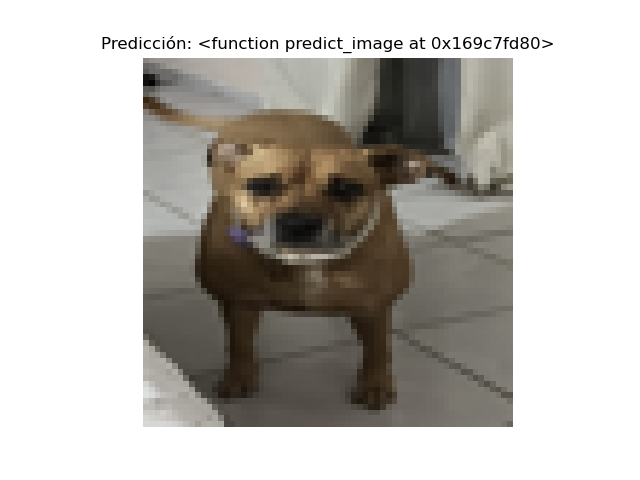
\includegraphics[width=.5\textwidth]{prediction_example.png}
    \caption{Ejemplo de predicción del modelo en imágenes nuevas.}
    \label{fig:predictions}
\end{figure}



\end{document}


